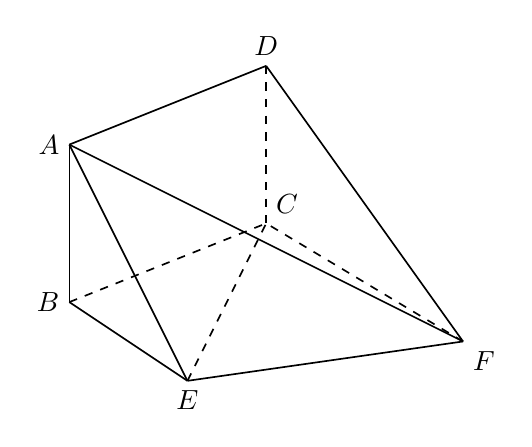
\begin{tikzpicture}[x=1cm,y=1cm,line width=0.6pt,font=\normalsize]
\coordinate (A) at (0,3);
\coordinate (D) at (2.5,4);
\coordinate (C) at (2.5,2);
\coordinate (B) at (0,1);
\coordinate (E) at (1.5,0);
\coordinate (F) at (5,0.5);
% solid edges
\draw (A) -- (D);
\draw (A) -- (B);
\draw (A) -- (E);
\draw (A) -- (F);
\draw (D) -- (F);
\draw (B) -- (E);
\draw (E) -- (F);
% hidden edges incident to C
\draw[dashed] (B) -- (C);
\draw[dashed] (D) -- (C);
\draw[dashed] (E) -- (C);
\draw[dashed] (F) -- (C);
% labels
\node[left] at (A) {$A$};
\node[above] at (D) {$D$};
\node[above right] at (C) {$C$};
\node[left] at (B) {$B$};
\node[below] at (E) {$E$};
\node[below right] at (F) {$F$};
\end{tikzpicture}
